% Options for packages loaded elsewhere
\PassOptionsToPackage{unicode}{hyperref}
\PassOptionsToPackage{hyphens}{url}
%
\documentclass[
  12pt,
]{article}
\title{County Level Predictors for Covid-19 Prevalence Before and After the Introduction of the Omicron Variant}
\author{Nathaniel Haulk\textsuperscript{1}}
\date{2021-12-08 16:17:28}

\usepackage{amsmath,amssymb}
\usepackage{lmodern}
\usepackage{setspace}
\usepackage{iftex}
\ifPDFTeX
  \usepackage[T1]{fontenc}
  \usepackage[utf8]{inputenc}
  \usepackage{textcomp} % provide euro and other symbols
\else % if luatex or xetex
  \usepackage{unicode-math}
  \defaultfontfeatures{Scale=MatchLowercase}
  \defaultfontfeatures[\rmfamily]{Ligatures=TeX,Scale=1}
\fi
% Use upquote if available, for straight quotes in verbatim environments
\IfFileExists{upquote.sty}{\usepackage{upquote}}{}
\IfFileExists{microtype.sty}{% use microtype if available
  \usepackage[]{microtype}
  \UseMicrotypeSet[protrusion]{basicmath} % disable protrusion for tt fonts
}{}
\makeatletter
\@ifundefined{KOMAClassName}{% if non-KOMA class
  \IfFileExists{parskip.sty}{%
    \usepackage{parskip}
  }{% else
    \setlength{\parindent}{0pt}
    \setlength{\parskip}{6pt plus 2pt minus 1pt}}
}{% if KOMA class
  \KOMAoptions{parskip=half}}
\makeatother
\usepackage{xcolor}
\IfFileExists{xurl.sty}{\usepackage{xurl}}{} % add URL line breaks if available
\IfFileExists{bookmark.sty}{\usepackage{bookmark}}{\usepackage{hyperref}}
\hypersetup{
  pdftitle={County Level Predictors for Covid-19 Prevalence Before and After the Introduction of the Omicron Variant},
  pdfauthor={Nathaniel Haulk1},
  hidelinks,
  pdfcreator={LaTeX via pandoc}}
\urlstyle{same} % disable monospaced font for URLs
\usepackage[margin=1in]{geometry}
\usepackage{longtable,booktabs,array}
\usepackage{calc} % for calculating minipage widths
% Correct order of tables after \paragraph or \subparagraph
\usepackage{etoolbox}
\makeatletter
\patchcmd\longtable{\par}{\if@noskipsec\mbox{}\fi\par}{}{}
\makeatother
% Allow footnotes in longtable head/foot
\IfFileExists{footnotehyper.sty}{\usepackage{footnotehyper}}{\usepackage{footnote}}
\makesavenoteenv{longtable}
\usepackage{graphicx}
\makeatletter
\def\maxwidth{\ifdim\Gin@nat@width>\linewidth\linewidth\else\Gin@nat@width\fi}
\def\maxheight{\ifdim\Gin@nat@height>\textheight\textheight\else\Gin@nat@height\fi}
\makeatother
% Scale images if necessary, so that they will not overflow the page
% margins by default, and it is still possible to overwrite the defaults
% using explicit options in \includegraphics[width, height, ...]{}
\setkeys{Gin}{width=\maxwidth,height=\maxheight,keepaspectratio}
% Set default figure placement to htbp
\makeatletter
\def\fps@figure{htbp}
\makeatother
% Make links footnotes instead of hotlinks:
\DeclareRobustCommand{\href}[2]{#2\footnote{\url{#1}}}
\setlength{\emergencystretch}{3em} % prevent overfull lines
\providecommand{\tightlist}{%
  \setlength{\itemsep}{0pt}\setlength{\parskip}{0pt}}
\setcounter{secnumdepth}{-\maxdimen} % remove section numbering
\newlength{\cslhangindent}
\setlength{\cslhangindent}{1.5em}
\newlength{\csllabelwidth}
\setlength{\csllabelwidth}{3em}
\newlength{\cslentryspacingunit} % times entry-spacing
\setlength{\cslentryspacingunit}{\parskip}
\newenvironment{CSLReferences}[2] % #1 hanging-ident, #2 entry spacing
 {% don't indent paragraphs
  \setlength{\parindent}{0pt}
  % turn on hanging indent if param 1 is 1
  \ifodd #1
  \let\oldpar\par
  \def\par{\hangindent=\cslhangindent\oldpar}
  \fi
  % set entry spacing
  \setlength{\parskip}{#2\cslentryspacingunit}
 }%
 {}
\usepackage{calc}
\newcommand{\CSLBlock}[1]{#1\hfill\break}
\newcommand{\CSLLeftMargin}[1]{\parbox[t]{\csllabelwidth}{#1}}
\newcommand{\CSLRightInline}[1]{\parbox[t]{\linewidth - \csllabelwidth}{#1}\break}
\newcommand{\CSLIndent}[1]{\hspace{\cslhangindent}#1}
\usepackage{geometry}
\geometry{verbose,letterpaper,margin=2.45cm}

% \usepackage[breaklinks=true,pdfstartview=FitH,citecolor=blue]{hyperref}
\hypersetup{colorlinks,%
	citecolor=blue,%
	filecolor=red,%
	linkcolor=blue,%
	urlcolor=red,%
	pdfstartview=FitH}

% \usepackage[T1]{fontenc}
% \usepackage[utf8]{inputenc}
% \usepackage{textgreek}
\usepackage{babel}
% % \usepackage{microtype}
% % \usepackage{amsmath}
\usepackage[osf]{libertine}
\usepackage{libertinust1math}
\usepackage{inconsolata}

\usepackage{longtable}

\usepackage{booktabs}

\usepackage{setspace}
% \doublespacing

% \setstretch{1.8999999999999999}

\usepackage{lineno}
% \linenumbers

\usepackage{flafter}
\usepackage{float}

% \renewcommand{\rmdefault}{cmr}

\usepackage[document]{ragged2e}

% % flush left while keep identation
% \makeatletter
% \newcommand\iraggedright{%
%   \let\\\@centercr\@rightskip\@flushglue \rightskip\@rightskip
%   \leftskip\z@skip}
% \makeatother
% \raggedright

% make pdf as default figure format
\DeclareGraphicsExtensions{.pdf,.png, %
    .jpg,.mps,.jpeg,.jbig2,.jb2,.JPG,.JPEG,.JBIG2,.JB2}
    
% \DeclareUnicodeCharacter{3B1}{\ensuremath{\alpha}}
% \DeclareUnicodeCharacter{3B2}{\ensuremath{\beta}}
% \DeclareUnicodeCharacter{0394}{$\Delta$}

\usepackage[labelsep=period]{caption}
\captionsetup{labelfont=bf}
% \usepackage{caption}
% \DeclareCaptionLabelSeparator{vline}{ \textbf{|} }
% \captionsetup{labelsep=vline, labelfont = {bf}}
\usepackage{booktabs}
\usepackage{longtable}
\usepackage{array}
\usepackage{multirow}
\usepackage{wrapfig}
\usepackage{float}
\usepackage{colortbl}
\usepackage{pdflscape}
\usepackage{tabu}
\usepackage{threeparttable}
\usepackage{threeparttablex}
\usepackage[normalem]{ulem}
\usepackage{makecell}
\usepackage{xcolor}
\ifLuaTeX
  \usepackage{selnolig}  % disable illegal ligatures
\fi

\begin{document}
\maketitle

% align only at left, not at right.
\renewcommand{\figurename}{{\textbf{Figure}}}
\renewcommand{\tablename}{{\textbf{Table}}}
% \iraggedright

\setstretch{1.5}
\footnotesize

\textsuperscript{1}Department of Biological Sciences, Louisiana State University, Baton Rouge, LA, USA

email: \href{mailto:nhaulk1@lsu.edu}{\nolinkurl{nhaulk1@lsu.edu}}; 232 Life Science Building, Baton Rouge, LA 70803

\normalsize

\textbf{Running headline}: Covid-19, Population Density, and the Omicron Variant

\textbf{Abstract}: Covid-19 rates may vary in rural and urban areas due to the resistance of many rural areas to partaking in preventative measures. The new variant of Covid-19, Omicron, may also disproportionately affect counties based on population size and the population density. Using records of cases per county, I compare the total cases in each county to the total population sizes. In addition, I compare the rate of infection in counties with and without mandates as well as rural versus urban counties. Finally, I calculate current effective reproductive rates with and without the introduction of the Omicron variant to the United States. Counties that had early mask mandates are seen with lower Covid-19 rates, and urban areas tend to have lower prevalence compared to rural areas. Northeastern counties are at the highest risk of Covid-19 infections with the addition of the Omicron variant exacerbating the effective reproductive number across the majority of counties. Precautionary measures should be taken know before the spread of the Omicron variant increases.

\clearpage

\hypertarget{introduction}{%
\section{Introduction}\label{introduction}}

The first case of Covid-19 was confirmed in the United States on January 20, 2020 according to the CDC (\protect\hyperlink{ref-cdc_cdc_2021}{CDC 2021a}). As of December 5, 2021, the United States had reported more than 780,000 deaths due to Covid-19, more than any other country (\protect\hyperlink{ref-new_york_times_coronavirus_2021}{New York Times 2021}). Initially, non-pharmaceutical methods were used to help stop the spread of Covid-19, including the closing of many public spaces, encouraging social distancing, and promoting the use of masks to help reduce transmission rates. Over time, social distancing and mask mandate policies changed as Covid-19 became the new norm, leading to patterns of increasing and decreasing Covid-19 rates in the United States (\protect\hyperlink{ref-rebeiro_impact_2021}{Rebeiro et al. 2021}). The current widespread availability of vaccines to fight Covid-19 has also helped to reduce the overall transmission and resulting mortality (\protect\hyperlink{ref-haas_infections_2021}{Haas et al. 2021}). Transmission and Covid-19 rates have increased post vaccination due to mutations in spike proteins that have allowed for new variants of COVID-19 to spread (\protect\hyperlink{ref-sheikh_sars-cov-2_2021}{Sheikh et al. 2021}, \protect\hyperlink{ref-monajjemi_delta_nodate}{Monajjemi et al. n.d.}). As of December 5th, 2021, the Delta variant is the most common strain of COVID-19, representing more than 99 percent of cases (\protect\hyperlink{ref-cdc_covid_2020}{CDC 2020}).

Mask mandates, social distancing, and vaccination have all been proven to reduce the transmission of Covid-19 (\protect\hyperlink{ref-ferguson_report_2020}{Ferguson et al. 2020}, \protect\hyperlink{ref-lyu_community_2020}{Lyu and Wehby 2020}, \protect\hyperlink{ref-nguyen_mask_2021}{Nguyen 2021}, \protect\hyperlink{ref-haas_infections_2021}{Haas et al. 2021}). Areas that adopted the use of masks early tended to have lower overall COVID-19 rates compared to those that did not. Given the efficacy of masks preventing transmission as well as the high availability to everyone, they have been one of the best tools in fighting the spread of Covid-19 (\protect\hyperlink{ref-rebeiro_impact_2021}{Rebeiro et al. 2021}). Despite the clear benefits, masks have been met with much opposition across the United States, especially in politically conservative leaning counties (\protect\hyperlink{ref-kahane_politicizing_2021}{Kahane 2021}, \protect\hyperlink{ref-he_why_2021}{He et al. 2021}). These counties tend to be more rural and more against mask mandates than their urban counterparts (\protect\hyperlink{ref-pro_us_2021}{Pro et al. 2021}).

Spatial heterogeneity, or the uneven distribution of populations across space, is important for predicting disease dynamics in pathogens like Covid-19. Areas with low spatial heterogeneity tend to be better environments for a disease to persist when compared to high spatial heterogeneous environments (\protect\hyperlink{ref-hagenaars_spatial_2004}{Hagenaars et al. 2004}). Populations with higher densities tend to have higher disease spread assuming the disease transmission is not based on frequency of contact (\protect\hyperlink{ref-scott_impact_1988}{Scott 1988}). Density dependent disease like Covid-19 should therefore have a harder time spreading in rural areas with higher heterogeneity and lower population densities. However, with resistance to preventative measures such as masks and vaccines, cases may be higher in rural areas than their urban counterparts (\protect\hyperlink{ref-sun_rural-urban_2021}{Sun and Monnat 2021}).

With changes in population density and spatial spread, the basic reproductive number, \(R_0\), should change as a result. The basic reproductive number represents the number of predicted infections that can result from one infection (\protect\hyperlink{ref-delamater_complexity_2019}{Delamater et al. 2019}). While studies have already looked into how \(R_0\) changes by county, no recent studies have looked at the effective reproductive number on a county level (\protect\hyperlink{ref-ives_estimating_2021}{Ives and Bozzuto 2021}). More importantly, not much is yet known about the new Omicron variant first introduced into the US on December 1, 2021. The Omicron variant is predicted to be more infectious than previous variants of Covid-19 and is predicted to be more resistant to the vaccines that are currently available (\protect\hyperlink{ref-cdc_omicron_2021}{CDC 2021b}). The reproductive number of the Omicron variant is not calculable at such a low prevalence due to the lack of data. However, predictions on how the new variant will spread provide vital information on preventing new infections and reducing overall mortality.

While data is presented on county-level Covid-19 rates, few studies have taken this further to investigate how the infection rates in urban and rural areas compare. With the Omicron variant just recently emerging, no studies have yet to been published examining the predicted rate of spread. In this study, I seek to investigate the total infection prevalence per county. I also compare the prevalence per county in rural and urban areas, as well as those with and without mask mandates. Finally, I seek to use previous predictions of \(R_0\) to calculate \(R_t\) in its current state. Using these current \(R_t\) values, I then infer predicted \(R_t\) values for Omicron for each county to highlight at-risk counties.

\hypertarget{methods}{%
\section{Methods}\label{methods}}

All code and graphs were written using the programming language R, and maps of the United States were modeled using the package USmaps (\protect\hyperlink{ref-lorenzo_usmap_2021}{Lorenzo 2021}, \protect\hyperlink{ref-r_core_team_r_2021}{R Core Team 2021}). For data on Covid-19 cases by county, I used the time series data provided by the \emph{New York Times} (\protect\hyperlink{ref-new_york_times_coronavirus_2021}{New York Times 2021}). For total population estimates, I used US Census data predictions for 2021 (\protect\hyperlink{ref-united_states_census_bureau_county_2021}{United States Census Bureau 2021a}). Total cases were mapped out as the number of cases in each county divided by the total population to get the total percentage of infections (Figure \ref{fig:fig1}). Rolling averages were mapped out based on reported cases within the last 30 days (Figure \ref{fig:fig2}). Mask mandate data used was collected in July of 2020 (\protect\hyperlink{ref-wright_tracking_2020}{Wright et al. 2020}). Data from the early infection was chosen and graphed to show how early responses to Covid-19 have led to differences in the total percentage of cases. A t-test was performed to test the significance between the two groups, and a bar graph was made for visualization (Figure \ref{fig:fig3}). Rural data was graphed using the HRSA criteria, where urban populations of urban areas have more than 50,000 individuals and rural areas have less than 50,000 (\protect\hyperlink{ref-hrsa_defining_2021}{HRSA 2021}). Census Bureau classifications were considered but led to few counties actually being classified as rural (\protect\hyperlink{ref-united_states_census_bureau_2010_2021}{United States Census Bureau 2021b}). This data was graphed as a map of the US to show county classification, as well as a bar graph to compare the average total case percentage (Figure \ref{fig:fig4}). A t-test was performed on the data classified based on the HRSA distinction of urban and rural to test for significance. Vaccine data was collected from the CDC to calculate the proportion of susceptible individuals (\protect\hyperlink{ref-cdc_covid-19_2021}{CDC 2021c}).

The effective reproductive number (\(R_t\)) was calculated using basic reproductive values (\(R_0\)) for each county predicted in a previous study (Figure \ref{fig:fig5}) (\protect\hyperlink{ref-ives_estimating_2021}{Ives and Bozzuto 2021}) . Using previous models and calculations of \(R_0\), the formula
\[R_0 = \frac{\beta*\lambda}{(\gamma+\mu+\epsilon+\sigma)*(\tau+\mu)}\]
was used to calculate the \(\beta\) value, or the transmission rate, per county (see Table \ref{tab:suptable1} for parameter descriptions) (\protect\hyperlink{ref-ahmed_mathematical_2021}{Ahmed et al. 2021}). Beta values were than used to calculate using the formula
\[R_t = (1-p)*\frac{S}{N}*\frac{\beta*\lambda}{(\gamma+\mu+\epsilon+\sigma)*(\tau+\mu)}\]
where S represents individuals susceptible to the disease and N represents the total population size in that count. Parameter p represents the proportion of vaccinated individuals per county (\protect\hyperlink{ref-cdc_covid-19_2021}{CDC 2021c}). The effective reproductive number for the Omicron variant was then calculated using the same formula, with higher overall transmission rates and lower mask usage to reflect the increase in \(R_0\) seen when the Delta variant of Covid-19 was first introduced into the United States (Figure \ref{fig:fig6}) (\protect\hyperlink{ref-liu_reproductive_2021}{Liu and Rocklöv 2021}).

\hypertarget{results}{%
\section{Results}\label{results}}

Counties varied considerably when comparing the total number of cases to the total population of that county (Figure \ref{fig:fig1}). One standout county is Chattahoochee County in Georgia, having the highest percentage of cases to total population size at almost 60\% of individuals having been infected. For the most part, the total percentage of cases seems to be relatively evenly distributed throughout states with occasional outliers. Average cases in the last thirty days adjusted for total population size show that the majority of cases occurred in the northeastern counties as well as in the midwestern counties (Figure \ref{fig:fig2}). Average cases tend to be relatively low in southern states, with the majority being near or at 0. This is due to a relatively large spike in cases that only have occurred in the South during the months of July through September (\protect\hyperlink{ref-new_york_times_coronavirus_2021}{New York Times 2021}).



\begin{figure}[H]

{\centering 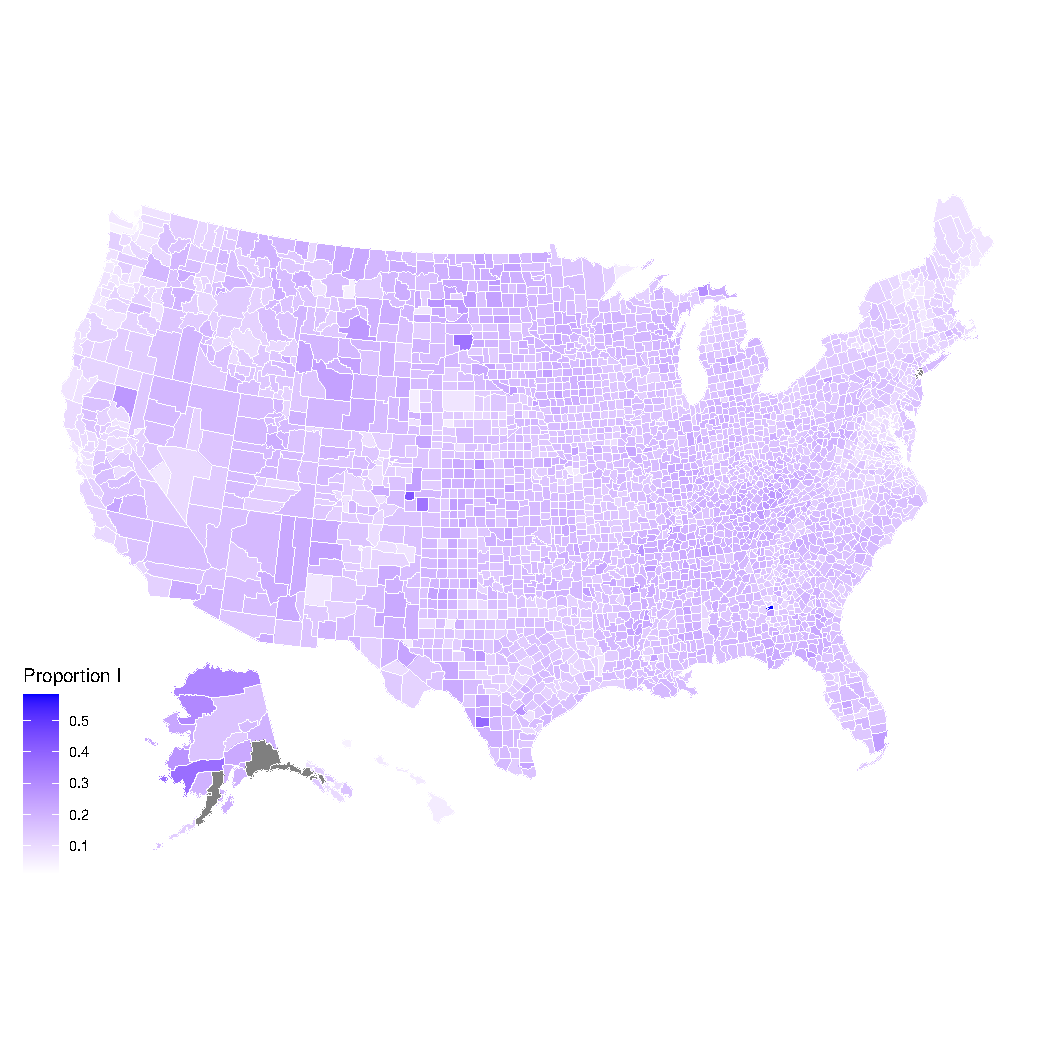
\includegraphics[width=0.7\linewidth,]{Final-Manuscript_files/figure-latex/fig1-1} 

}

\caption{Total cases divided by the total population per county. Counties with the highest case rate are a darker blue color.}\label{fig:fig1}
\end{figure}



\begin{figure}[H]

{\centering 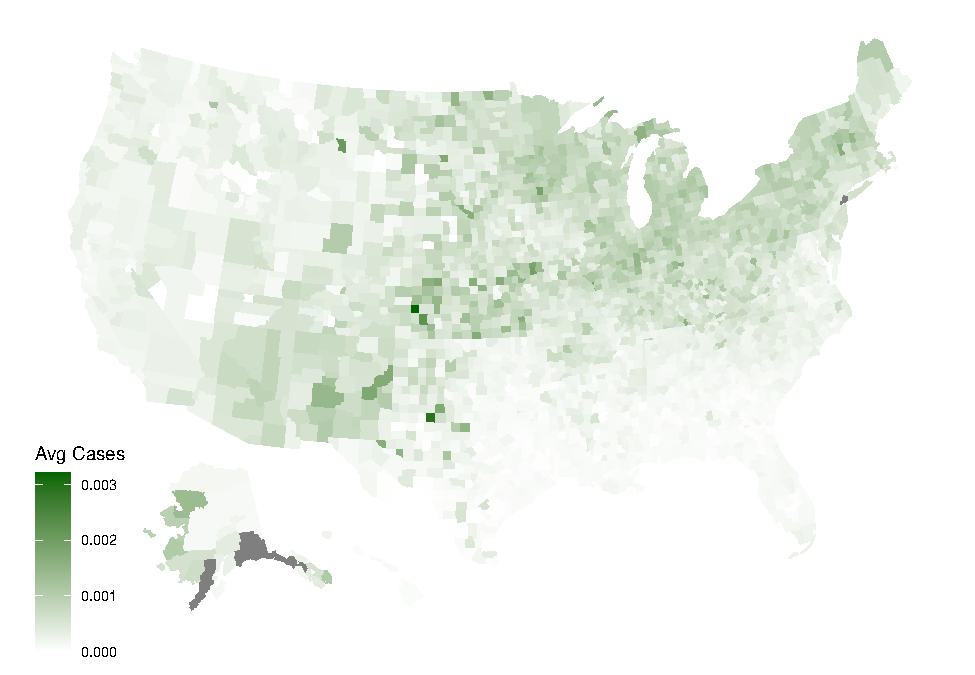
\includegraphics[width=0.7\linewidth,]{Final-Manuscript_files/figure-latex/fig2-1} 

}

\caption{Average number of cases in the past thirty days divided by the total population per county. Counties with the highest case rate are a dark green color.}\label{fig:fig2}
\end{figure}

Mask data showed a predictable pattern where early adopters of mask mandates tended to have lower overall total prevalence. Counties that adopted early mask mandates had an average total prevalence of 0.155 while counties that did not adopt masks early had an average total prevalence of 0.17. The difference is significant with a p-value of 1.00623095289842e-31 (Figure \ref{fig:fig3}b). Mapping out rural vs urban areas by populations unsurprisingly shows that the urban areas tend to center around large cities or states with high overall populations like the majority of counties in the Northeast and along the coast of California (Figure \ref{fig:fig4}a). Overall, rural counties tended to have a higher average total infection prevalence of 0.167, while urban areas had an average total infection prevalence of 0.153 The difference between the urban and rural areas was significant with a p-value of 1.21849570897781e-25.



\begin{figure}[H]

{\centering 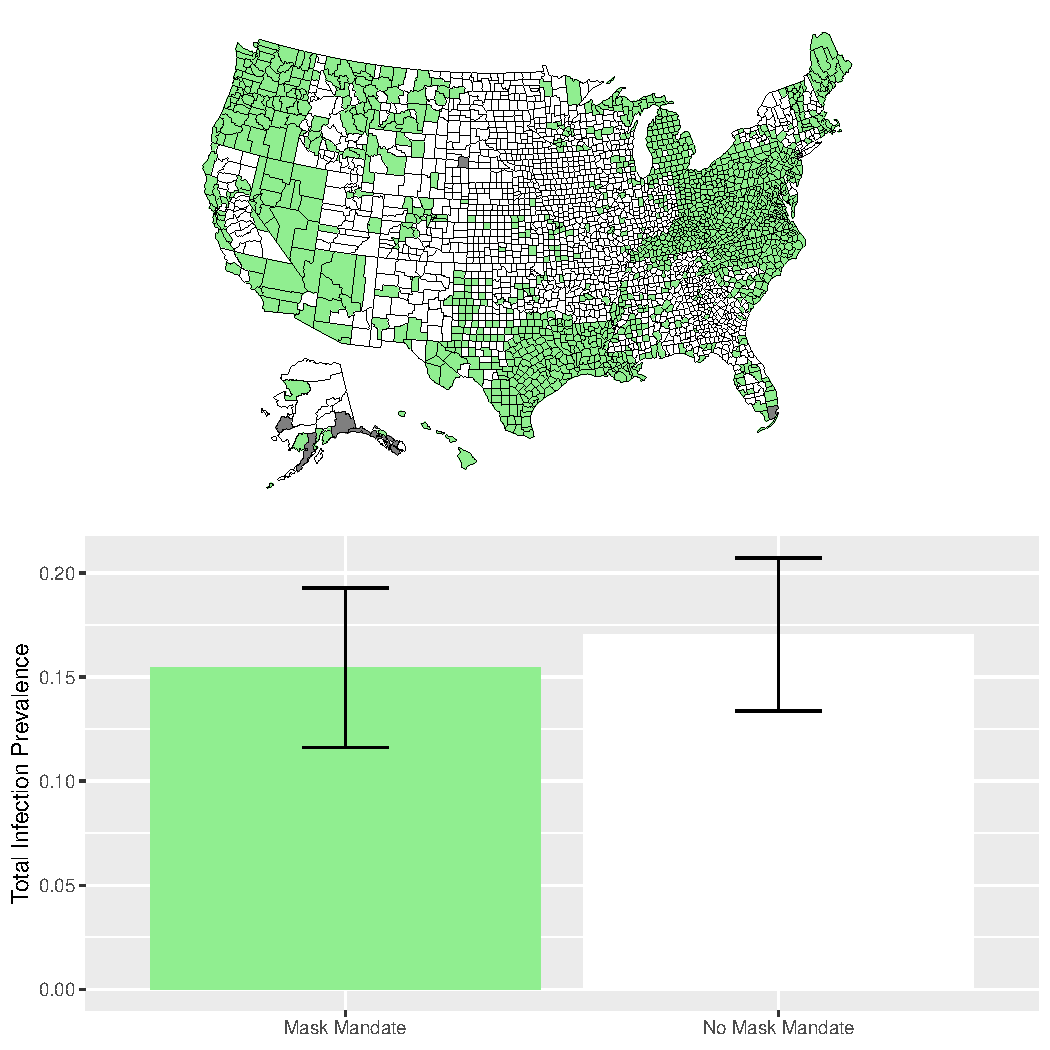
\includegraphics{Final-Manuscript_files/figure-latex/fig3-1} 

}

\caption{\textbf{a)} The counties that adopted mask mandates during the early stages of the pandemic highlighted in green. Counties highlighted in white did not adopt mask mandates. \textbf{b)} The average percentage of infection in counties with and without mask mandates (p = 1.00623095289842e-31).}\label{fig:fig3}
\end{figure}



\begin{figure}[H]

{\centering 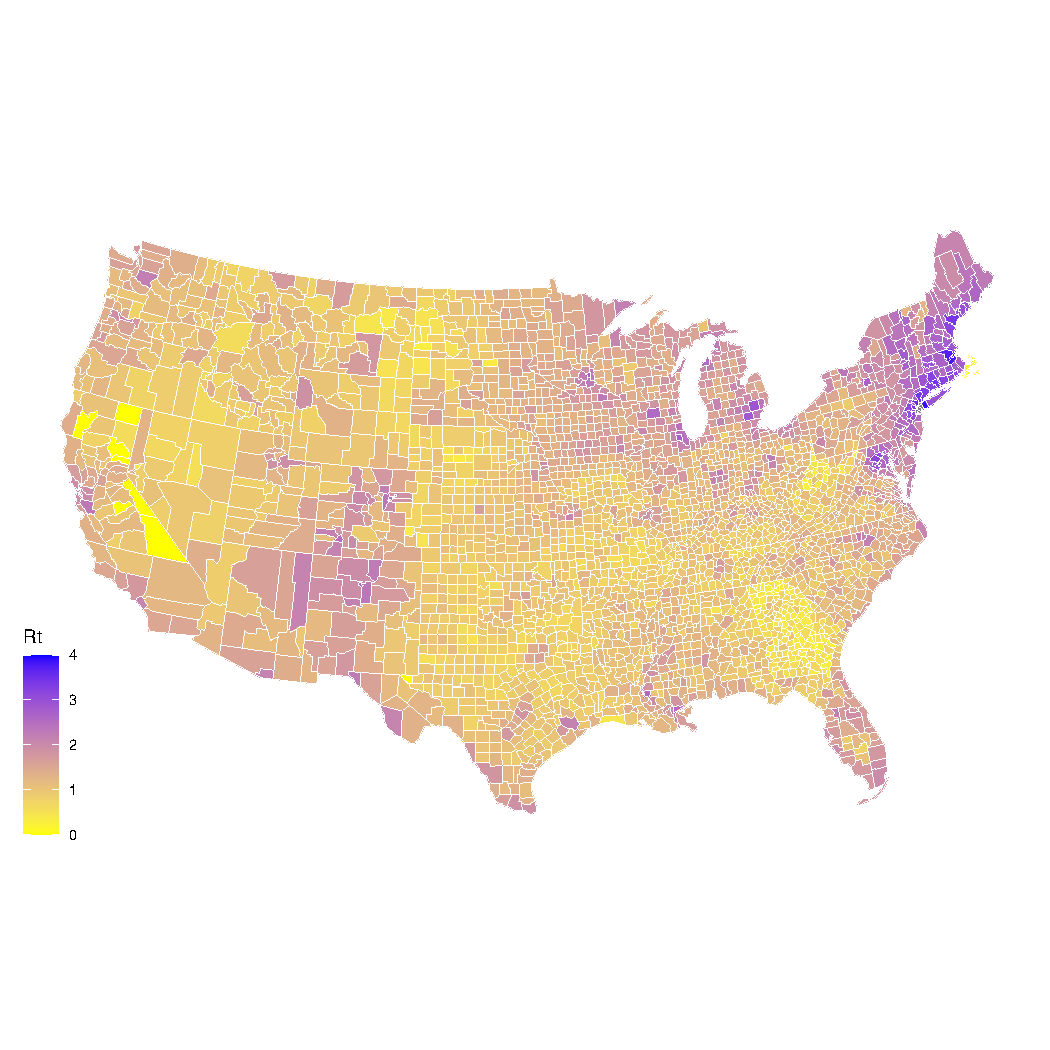
\includegraphics{Final-Manuscript_files/figure-latex/fig4-1} 

}

\caption{\textbf{a)} The counties highlighted in red are considered urban. Counties highlighted in white are considered rural. \textbf{b)} The average percentage of infection in counties considered rural compared to the counties considered urban (p = 1.21849570897781e-25).}\label{fig:fig4}
\end{figure}

Using previously calculated \(R_0\) to derive beta, I calculated the predictive effective reproductive number for each county (Figure \ref{fig:fig5}). Numerous counties, especially in the state of Georgia, have actually reached an \(R_0\) value below 1, meaning that the disease will eventually go extinct in the long term in these areas. The average effective reproductive number across all counties is 0.78. However, the effective reproductive number is still relatively high in the northeastern parts of the United States. The addition of the Omicron variant shows an expected increase of the effective reproductive number in almost every county (Figure \ref{fig:fig6}). When the Omicron variant is included, the average effective reproductive number increases to an average of 1.243.



\begin{figure}[H]

{\centering 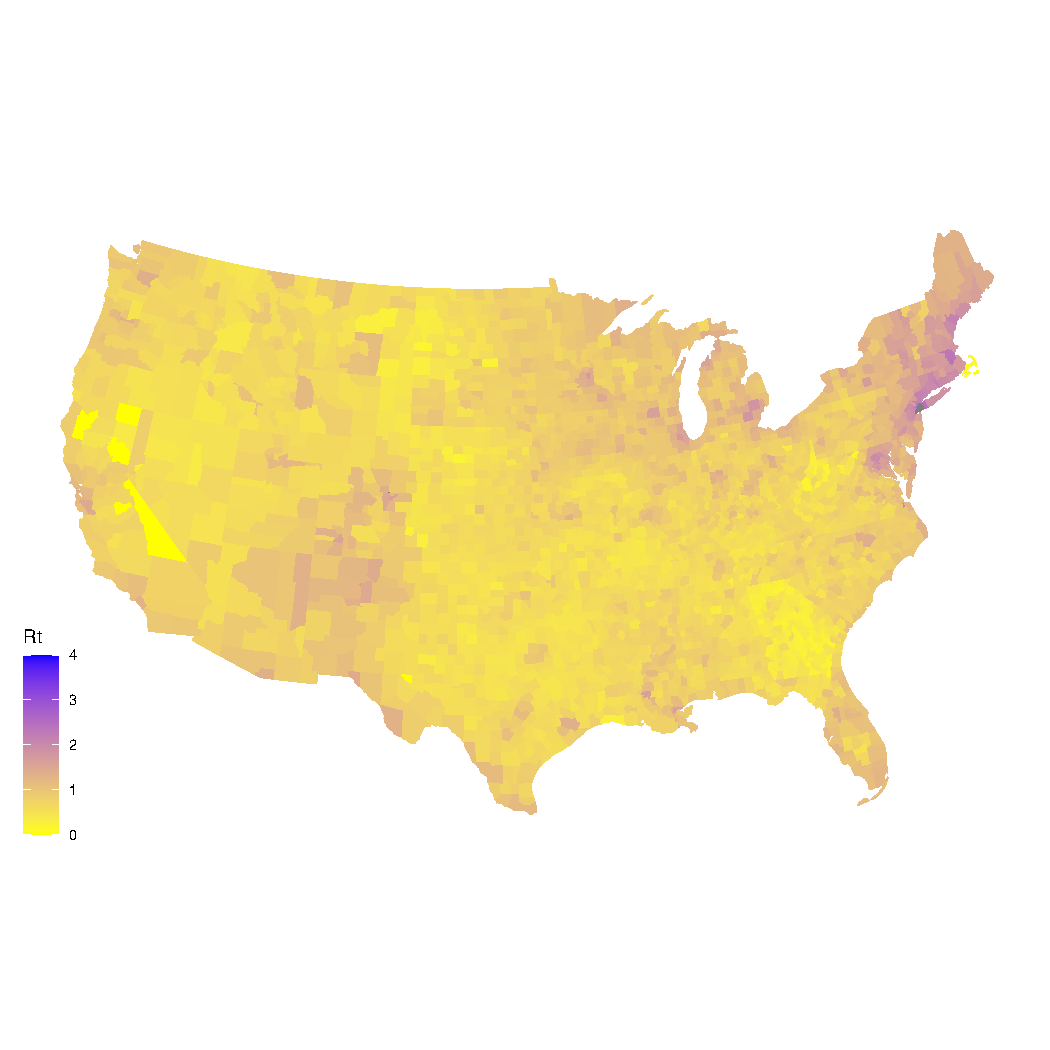
\includegraphics{Final-Manuscript_files/figure-latex/fig5-1} 

}

\caption{The effective reproductive number for each county as of 12/5/2021. Counties in bright yellow have an \(R_0\) below 1 and will therefore see a decline and eventual extinction of the pathogen.}\label{fig:fig5}
\end{figure}



\begin{figure}[H]

{\centering 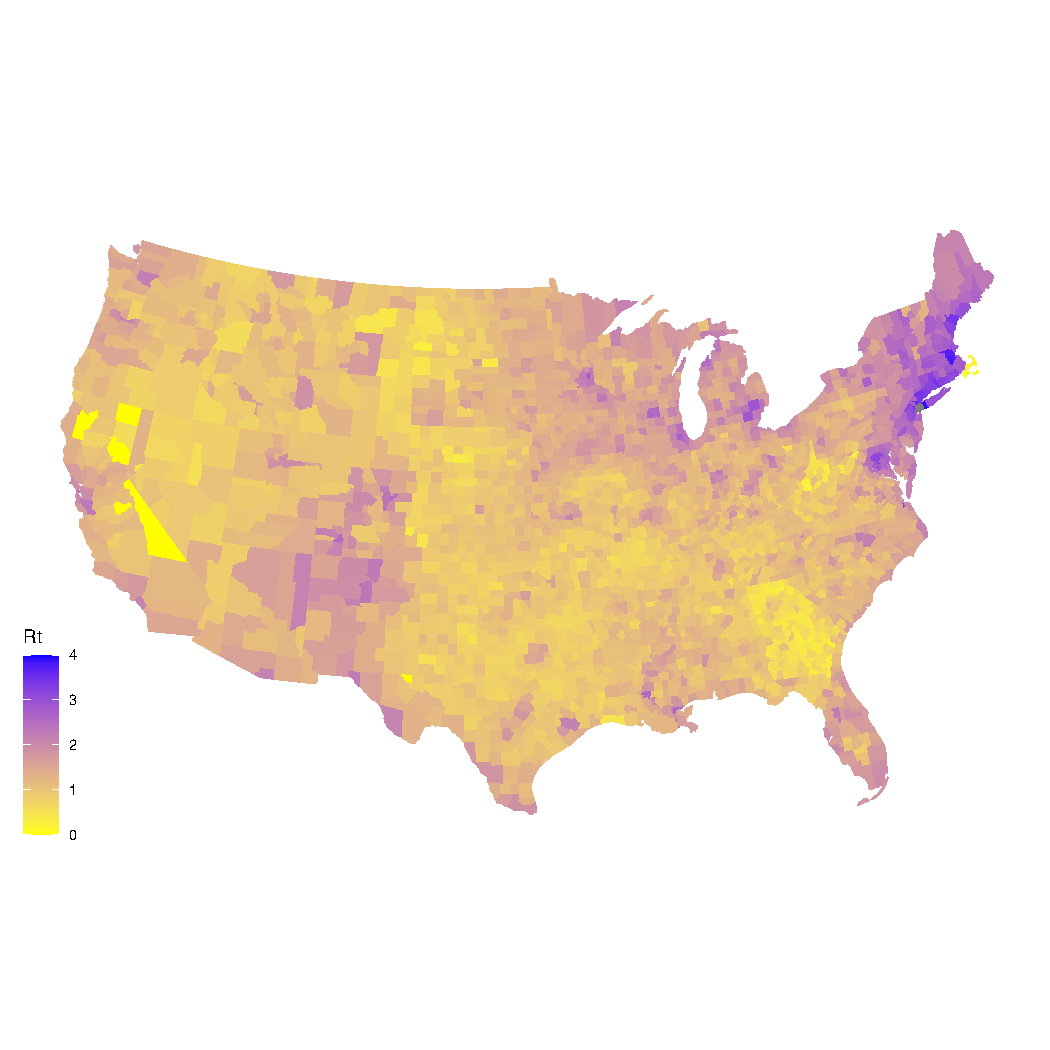
\includegraphics{Final-Manuscript_files/figure-latex/fig6-1} 

}

\caption{The predicted effective reproductive number for each county as of 12/5/2021, assuming the Omicron variant is as transmissible as predicted. Counties in bright yellow have an \(R_0\) below 1 and will therefore see a decline and eventual extinction of the pathogen. While the northeast continues to have the highest potential for disease spread, other areas that were not as at risk originally now have more concerning effective reproductive numbers.}\label{fig:fig6}
\end{figure}

\hypertarget{discussion}{%
\section{Discussion}\label{discussion}}

While work looking into Covid-19 dynamics on a county level has been completed in the past, little work has been performed after the introduction of the vaccine and with our current knowledge of the pathogen. Here I show that early mask mandates were an important response to keeping cases low. This result is in line with other studies that have compared mask requirements at a state level and found that states with higher mask use tended to have lower cases (\protect\hyperlink{ref-white_state-level_2020}{White and Hébert-Dufresne 2020}). Despite the assumption that Covid-19 has a higher transmission rate in more densely populated areas and how Covid-19 has been shown to spread in other countries, the United States seems to have higher case rates in rural, less populated areas (\protect\hyperlink{ref-rader_crowding_2020}{Rader et al. 2020}). This is most likely due to the behavior of individuals within these areas as well as resistance to mask mandates and other preventative measures (\protect\hyperlink{ref-pro_us_2021}{Pro et al. 2021}). It may also be due in part to the fact that more densely populated areas tend to have more intervention from the government in terms of preventative measures.

Across the United States, effective reproductive values were on average below 1. This means that many parts of the country are close to herd immunity (\protect\hyperlink{ref-fine_herd_2011}{Fine et al. 2011}). Areas of concern are counties in the Northeast, the area with the highest effective reproductive number. Shortages of medical equipment like ventilators have caused issues for hospitals and interfered with proper care of patients in the past (\protect\hyperlink{ref-sen-crowe_closer_2021}{Sen-Crowe et al. 2021}). Based on these values, equipment should be made more readily available to hospitals in the Northeast as these populations are the most vulnerable. In addition, individuals in these areas should be further encouraged to receive the vaccine to help prevent future cases.

If Omicron is as infectious as currently predicted, counties across the country are at a much higher risk of contracting Covid-19 (\protect\hyperlink{ref-cdc_omicron_2021}{CDC 2021b}). To help reduce the potential strain Omicron will have on medical centers, mask mandates and other preventative measures should be implemented again, especially in areas like the northeastern part of the United States where the predicted effective reproductive number is high. Preliminary studies suggest that vaccines also provide some protection against the Omicron variant (\protect\hyperlink{ref-zimmer_covid_2021}{Zimmer and Mueller 2021}). Pushing for vaccines in these areas can further help reduce the spread of the disease. While new information is discovered on Omicron every day and the variant may not be as serious as previously predicted, news is lacking, and data is often based on anecdotes or studies with small sample sizes (\protect\hyperlink{ref-callaway_how_2021}{Callaway and Ledford 2021}). Preventative measures should be taken regardless in order to reduce mortality in case this variant is more severe than predicted.

There are several limitations to this study that require future work. For starters, the size of the county is not taken into effect. Some counties, especially in areas like New Mexico and Arizona, are considered urban due to their sheer size and not necessarily due to their population density. Another limitation is how data is recorded and presented on a county level. I currently assume that cases are the best representations of Covid-19 data. However, since Covid tests can report false positives, using excess death data may give a better estimate of the actual rates of Covid-19 in each county. Reporting is not consistent across the United States, with many areas like Florida inconsistently reporting data. Further work could investigate how movement between counties may lead to changing the effective reproductive number, as well as further investigate the dynamics of the Omicron variant once more is known.

\hypertarget{conclusion}{%
\subsection{Conclusion}\label{conclusion}}

I found a significant difference between the total Covid-19 prevalence in rural and urban areas, with urban areas trending towards lower overall prevalence than rural. Counties that did not adopt early mask mandates unsurprisingly showed higher rates of Covid-19 than those who did. Predictions based on current data on the Omicron variant show that almost all counties will be susceptible to the increased transmission caused by the variant, and resources should especially be focused on the Northeast where the effective reproductive number is predicted to be the highest. More work needs to be done once additional data is gathered on the Omicron variant to properly model and predict the most at-risk counties for further intervention.

\hypertarget{references}{%
\section{References}\label{references}}

\hypertarget{refs}{}
\begin{CSLReferences}{1}{0}
\leavevmode\vadjust pre{\hypertarget{ref-ahmed_mathematical_2021}{}}%
Ahmed, I., G. U. Modu, A. Yusuf, P. Kumam, and I. Yusuf. 2021. A mathematical model of {Coronavirus} {Disease} ({COVID}-19) containing asymptomatic and symptomatic classes. Results in Physics 21:103776.

\leavevmode\vadjust pre{\hypertarget{ref-callaway_how_2021}{}}%
Callaway, E., and H. Ledford. 2021. How bad is {Omicron}? {What} scientists know so far. Nature 600:197--199.

\leavevmode\vadjust pre{\hypertarget{ref-cdc_covid_2020}{}}%
CDC. 2020, March. {COVID} {Data} {Tracker}.

\leavevmode\vadjust pre{\hypertarget{ref-cdc_cdc_2021}{}}%
CDC. 2021a, August. {CDC} {Museum} {COVID}-19 {Timeline}.

\leavevmode\vadjust pre{\hypertarget{ref-cdc_omicron_2021}{}}%
CDC. 2021b, December. Omicron {Variant}: {What} {You} {Need} to {Know}.

\leavevmode\vadjust pre{\hypertarget{ref-cdc_covid-19_2021}{}}%
CDC. 2021c, December. {COVID}-19 {Vaccinations} in the {United} {States},{County} {\textbar} {Data} {\textbar} {Centers} for {Disease} {Control} and {Prevention}.

\leavevmode\vadjust pre{\hypertarget{ref-delamater_complexity_2019}{}}%
Delamater, P. L., E. J. Street, T. F. Leslie, Y. T. Yang, and K. H. Jacobsen. 2019. Complexity of the {Basic} {Reproduction} {Number} ({R0}). Emerging Infectious Diseases 25:1--4.

\leavevmode\vadjust pre{\hypertarget{ref-ferguson_report_2020}{}}%
Ferguson, N., D. Laydon, G. Nedjati Gilani, N. Imai, K. Ainslie, M. Baguelin, S. Bhatia, A. Boonyasiri, Z. Cucunuba Perez, G. Cuomo-Dannenburg, A. Dighe, I. Dorigatti, H. Fu, K. Gaythorpe, W. Green, A. Hamlet, W. Hinsley, L. Okell, S. Van Elsland, H. Thompson, R. Verity, E. Volz, H. Wang, Y. Wang, P. Walker, P. Winskill, C. Whittaker, C. Donnelly, S. Riley, and A. Ghani. 2020. Report 9: {Impact} of non-pharmaceutical interventions ({NPIs}) to reduce {COVID19} mortality and healthcare demand. Imperial College London.

\leavevmode\vadjust pre{\hypertarget{ref-fine_herd_2011}{}}%
Fine, P., K. Eames, and D. L. Heymann. 2011. {``{Herd} {Immunity}''}: {A} {Rough} {Guide}. Clinical Infectious Diseases 52:911--916.

\leavevmode\vadjust pre{\hypertarget{ref-haas_infections_2021}{}}%
Haas, E. J., J. M. McLaughlin, F. Khan, F. J. Angulo, E. Anis, M. Lipsitch, S. R. Singer, G. Mircus, N. Brooks, M. Smaja, K. Pan, J. Southern, D. L. Swerdlow, L. Jodar, Y. Levy, and S. Alroy-Preis. 2021. Infections, hospitalisations, and deaths averted via a nationwide vaccination campaign using the {Pfizer}--{BioNTech} {BNT162b2} {mRNA} {COVID}-19 vaccine in {Israel}: A retrospective surveillance study. The Lancet Infectious Diseases.

\leavevmode\vadjust pre{\hypertarget{ref-hagenaars_spatial_2004}{}}%
Hagenaars, T. J., C. A. Donnelly, and N. M. Ferguson. 2004. Spatial heterogeneity and the persistence of infectious diseases. Journal of Theoretical Biology 229:349--359.

\leavevmode\vadjust pre{\hypertarget{ref-he_why_2021}{}}%
He, L., C. He, T. L. Reynolds, Q. Bai, Y. Huang, C. Li, K. Zheng, and Y. Chen. 2021. Why do people oppose mask wearing? {A} comprehensive analysis of {U}.{S}. Tweets during the {COVID}-19 pandemic. Journal of the American Medical Informatics Association : JAMIA 28:1564--1573.

\leavevmode\vadjust pre{\hypertarget{ref-hrsa_defining_2021}{}}%
HRSA. 2021, October. Defining {Rural} {Population}. Text.

\leavevmode\vadjust pre{\hypertarget{ref-ives_estimating_2021}{}}%
Ives, A. R., and C. Bozzuto. 2021. Estimating and explaining the spread of {COVID}-19 at the county level in the {USA}. Communications Biology 4:60.

\leavevmode\vadjust pre{\hypertarget{ref-kahane_politicizing_2021}{}}%
Kahane, L. H. 2021. Politicizing the {Mask}: {Political}, {Economic} and {Demographic} {Factors} {Affecting} {Mask} {Wearing} {Behavior} in the {USA}. Eastern Economic Journal 47:163--183.

\leavevmode\vadjust pre{\hypertarget{ref-liu_reproductive_2021}{}}%
Liu, Y., and J. Rocklöv. 2021. The reproductive number of the {Delta} variant of {SARS}-{CoV}-2 is far higher compared to the ancestral {SARS}-{CoV}-2 virus. Journal of Travel Medicine 28:taab124.

\leavevmode\vadjust pre{\hypertarget{ref-lorenzo_usmap_2021}{}}%
Lorenzo, P. D. 2021. Usmap: {US} {Maps} {Including} {Alaska} and {Hawaii}.

\leavevmode\vadjust pre{\hypertarget{ref-lyu_community_2020}{}}%
Lyu, W., and G. L. Wehby. 2020. Community {Use} {Of} {Face} {Masks} {And} {COVID}-19: {Evidence} {From} {A} {Natural} {Experiment} {Of} {State} {Mandates} {In} {The} {US}. Health Affairs 39:1419--1425.

\leavevmode\vadjust pre{\hypertarget{ref-monajjemi_delta_nodate}{}}%
Monajjemi, M., F. Kandemirli, and F. Mollaamin. (n.d.). Delta {Variant} of {Covid}-19 {Study}, and {Why} it is a {Concern}: {An} {Overview}:14.

\leavevmode\vadjust pre{\hypertarget{ref-new_york_times_coronavirus_2021}{}}%
New York Times. 2021, December. Coronavirus ({Covid}-19) {Data} in the {United} {States}. The New York Times.

\leavevmode\vadjust pre{\hypertarget{ref-nguyen_mask_2021}{}}%
Nguyen, M. 2021. Mask {Mandates} and {COVID}-19 {Related} {Symptoms} in the {US}. ClinicoEconomics and Outcomes Research: CEOR 13:757--766.

\leavevmode\vadjust pre{\hypertarget{ref-pro_us_2021}{}}%
Pro, G., K. Schumacher, R. Hubach, N. Zaller, Z. Giano, R. Camplain, C. Camplain, S. Haberstroh, J. A. Baldwin, and D. L. Wheeler. 2021. {US} trends in mask wearing during the {COVID}-19 pandemic depend on rurality. Rural Remote Health:6596--6596.

\leavevmode\vadjust pre{\hypertarget{ref-r_core_team_r_2021}{}}%
R Core Team. 2021. R: {A} {Language} and {Environment} for {Statistical} {Computing}. R Foundation for Statistical Computing, Vienna, Austria.

\leavevmode\vadjust pre{\hypertarget{ref-rader_crowding_2020}{}}%
Rader, B., A. Nande, B. Adlam, A. L. Hill, R. C. Reiner, D. M. Pigott, B. Gutierrez, COVID-19 data working group, J. S. Brownstein, M. C. Castro, H. Tian, O. G. Pybus, S. V. Scarpino, and M. U. Kraemer. 2020. Crowding and the epidemic intensity of {COVID}-19 transmission. preprint, Epidemiology.

\leavevmode\vadjust pre{\hypertarget{ref-rebeiro_impact_2021}{}}%
Rebeiro, P. F., D. M. Aronoff, and M. K. Smith. 2021. The {Impact} of {State} {Mask}-{Wearing} {Requirements} on the {Growth} of {Coronavirus} {Disease} 2019 {Cases}, {Hospitalizations}, and {Deaths} in the {United} {States}. Clinical Infectious Diseases 73:1703--1706.

\leavevmode\vadjust pre{\hypertarget{ref-scott_impact_1988}{}}%
Scott, M. E. 1988. The {Impact} of {Infection} and {Disease} on {Animal} {Populations}: {Implications} for {Conservation} {Biology}. Conservation Biology 2:40--56.

\leavevmode\vadjust pre{\hypertarget{ref-sen-crowe_closer_2021}{}}%
Sen-Crowe, B., M. Sutherland, M. McKenney, and A. Elkbuli. 2021. A {Closer} {Look} {Into} {Global} {Hospital} {Beds} {Capacity} and {Resource} {Shortages} {During} the {COVID}-19 {Pandemic}. Journal of Surgical Research 260:56--63.

\leavevmode\vadjust pre{\hypertarget{ref-sheikh_sars-cov-2_2021}{}}%
Sheikh, A., J. McMenamin, B. Taylor, and C. Robertson. 2021. {SARS}-{CoV}-2 {Delta} {VOC} in {Scotland}: Demographics, risk of hospital admission, and vaccine effectiveness. The Lancet 397:2461--2462.

\leavevmode\vadjust pre{\hypertarget{ref-sun_rural-urban_2021}{}}%
Sun, Y., and S. M. Monnat. 2021. Rural-urban and within-rural differences in {COVID}-19 vaccination rates. The Journal of Rural Health n/a.

\leavevmode\vadjust pre{\hypertarget{ref-united_states_census_bureau_county_2021}{}}%
United States Census Bureau. 2021a. County {Population} {Totals}: 2010-2020.

\leavevmode\vadjust pre{\hypertarget{ref-united_states_census_bureau_2010_2021}{}}%
United States Census Bureau. 2021b, October. 2010 {Census} {Urban} and {Rural} {Classification} and {Urban} {Area} {Criteria}.

\leavevmode\vadjust pre{\hypertarget{ref-white_state-level_2020}{}}%
White, E. R., and L. Hébert-Dufresne. 2020. State-level variation of initial {COVID}-19 dynamics in the {United} {States}. PLOS ONE 15:e0240648.

\leavevmode\vadjust pre{\hypertarget{ref-wright_tracking_2020}{}}%
Wright, A. L., G. Chawla, L. Chen, and A. Farmer. 2020. Tracking {Mask} {Mandates} {During} the {Covid}-19 {Pandemic}. SSRN Electronic Journal.

\leavevmode\vadjust pre{\hypertarget{ref-zimmer_covid_2021}{}}%
Zimmer, C., and B. Mueller. 2021. Covid {Updates}: {Early} {Study} {Shows} {Pfizer} {Vaccine} {Gives} {Some} {Protection} {Against} {Omicron}. The New York Times.

\end{CSLReferences}

\clearpage

\setcounter{page}{0}
\pagenumbering{arabic}
\setcounter{page}{1}

\setcounter{figure}{0}
\setcounter{table}{0}
\renewcommand {\thetable}{S\arabic{table}}
\renewcommand {\thefigure}{S\arabic{figure}}

\hypertarget{supporting-information}{%
\section{Supporting Information}\label{supporting-information}}

\hypertarget{tables}{%
\subsection{Tables}\label{tables}}

\begin{longtable}[]{@{}lcc@{}}
\caption{\label{tab:suptable1} Parameter descriptions and values used to calculate \(R_0\) (\protect\hyperlink{ref-ahmed_mathematical_2021}{Ahmed et al. 2021}).}\tabularnewline
\toprule
Parameter & Value & Description \\
\midrule
\endfirsthead
\toprule
Parameter & Value & Description \\
\midrule
\endhead
\(\beta\) & Varies & Transmission rate \\
\(\lambda\) & \(.0025\) & Births into system \\
\(\gamma\) & \(2.01*10^{-4}\) & Transfer from the exposed class to the quarantined class \\
\(\mu\) & \(.0015\) & Natural Mortality Rate \\
\(\epsilon\) & \(.45\) & Transfer from the exposed class to the symptomatic infected class \\
\(\sigma\) & \(.067\) & Transfer from the exposed class to the asymptomatic infected class \\
\(\tau\) & \(2*10^{-4}\) & Transfer from the susceptible class to the quarantine class \\
p & Varies & Proportion vaccinated \\
\bottomrule
\end{longtable}

\end{document}
